\documentclass[border=12pt,tikz]{standalone}
\usepackage{fontspec}
\setmainfont{Helvetica Neue}
\setsansfont{Helvetica Neue}
\setmonofont{Menlo}
\usepackage{tikz}
\usetikzlibrary{positioning, arrows.meta, fit, backgrounds, calc, decorations.pathreplacing, matrix}

\definecolor{particle}{HTML}{E3F2FD}
\definecolor{particleborder}{HTML}{2196F3}
\definecolor{batch}{HTML}{E8F5E9}
\definecolor{batchborder}{HTML}{4CAF50}
\definecolor{handler}{HTML}{FFF3E0}
\definecolor{handlerborder}{HTML}{FF9800}
\definecolor{gray50}{HTML}{9E9E9E}
\definecolor{accent}{HTML}{7B1FA2}

\begin{document}
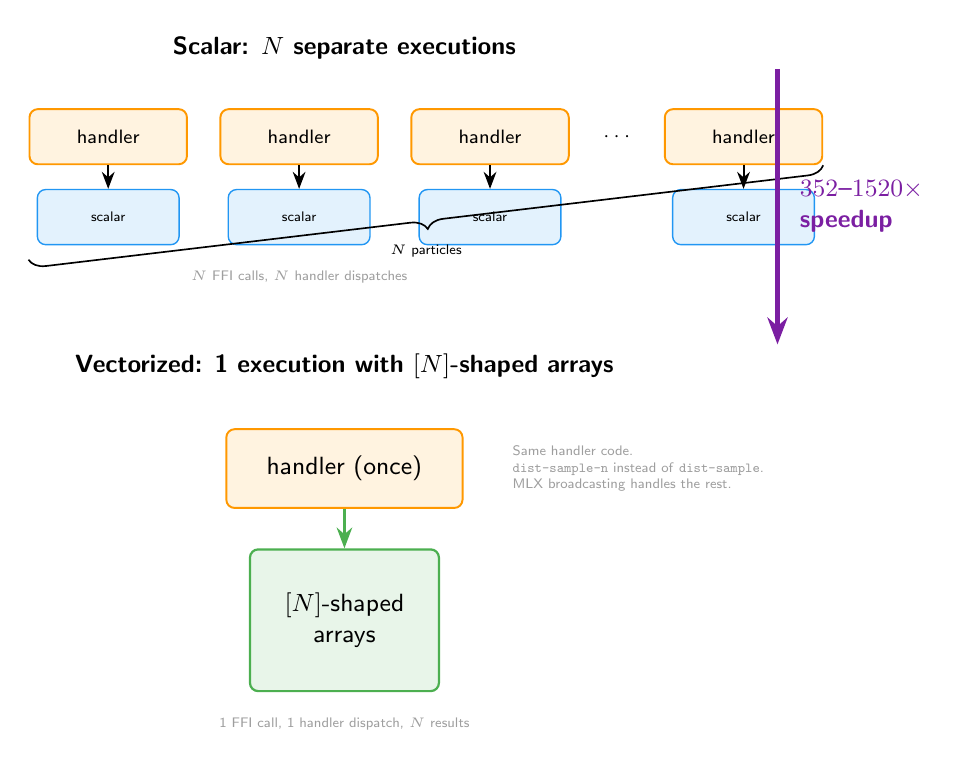
\begin{tikzpicture}[
    >=Stealth,
    node distance=0.5cm and 1cm,
    pbox/.style={draw, rounded corners=3pt, minimum height=0.7cm, minimum width=1.8cm,
                 font=\sffamily\tiny, fill=particle, draw=particleborder, line width=0.5pt},
    batchbox/.style={draw, rounded corners=3pt, minimum height=1.8cm, minimum width=2.4cm,
                     font=\sffamily\small, fill=batch, draw=batchborder, line width=0.8pt, align=center},
    hbox/.style={draw, rounded corners=3pt, minimum height=0.7cm, minimum width=2cm,
                 font=\sffamily\scriptsize, fill=handler, draw=handlerborder, line width=0.7pt},
    secheader/.style={font=\sffamily\small\bfseries},
    label/.style={font=\sffamily\tiny, color=gray50},
    arrow/.style={->, line width=0.7pt},
]

% ============================================================
% SCALAR (top): N separate executions
% ============================================================
\node[secheader] (scalar-title) {Scalar: $N$ separate executions};

% N handler boxes
\node[hbox, below=0.5cm of scalar-title, xshift=-3cm] (h1) {handler};
\node[hbox, right=0.4cm of h1] (h2) {handler};
\node[hbox, right=0.4cm of h2] (h3) {handler};
\node[font=\sffamily\scriptsize, right=0.3cm of h3] (dots1) {$\cdots$};
\node[hbox, right=0.3cm of dots1] (hN) {handler};

% Scalar values below
\node[pbox, below=0.3cm of h1] (v1) {scalar};
\node[pbox, below=0.3cm of h2] (v2) {scalar};
\node[pbox, below=0.3cm of h3] (v3) {scalar};
\node[pbox, below=0.3cm of hN] (vN) {scalar};

\draw[arrow] (h1) -- (v1);
\draw[arrow] (h2) -- (v2);
\draw[arrow] (h3) -- (v3);
\draw[arrow] (hN) -- (vN);

\node[label, below=0.2cm of v2] {$N$ FFI calls, $N$ handler dispatches};

% Brace showing N
\draw[decorate, decoration={brace, amplitude=6pt, mirror}, line width=0.6pt]
    (h1.south west) ++(0,-1.2cm) -- (hN.south east) ++(0,-1.2cm)
    node[midway, below=8pt, font=\sffamily\tiny] {$N$ particles};

% ============================================================
% VECTORIZED (bottom): 1 execution with [N]-shaped arrays
% ============================================================
\node[secheader, below=3.5cm of scalar-title] (vec-title) {Vectorized: 1 execution with $[N]$-shaped arrays};

% One handler box
\node[hbox, below=0.5cm of vec-title, minimum width=3cm, minimum height=1cm,
      font=\sffamily\small] (hvec) {handler (once)};

% [N]-shaped array below
\node[batchbox, below=0.5cm of hvec] (bvec) {$[N]$-shaped\\arrays};

% Individual values inside the batch box (visual hint)
\draw[arrow, line width=1pt, color=batchborder] (hvec) -- (bvec);

% Arrow showing broadcasting
\node[label, right=0.5cm of hvec, align=left, text width=4.5cm] {
  Same handler code.\\
  \texttt{dist-sample-n} instead of \texttt{dist-sample}.\\
  MLX broadcasting handles the rest.
};

\node[label, below=0.2cm of bvec] {1 FFI call, 1 handler dispatch, $N$ results};

% Speedup annotation
\draw[->, line width=1.5pt, color=accent] ([xshift=5.5cm]scalar-title.south) -- ([xshift=5.5cm]vec-title.north)
    node[midway, right=4pt, font=\sffamily\small\bfseries, color=accent, align=left] {$352$--$1520\times$\\speedup};

\end{tikzpicture}
\end{document}
